\subsection{Xây dựng mô-đun ghép từ thành câu tiếng Việt}

Nếu Chương 2 tập trung vào việc giải thích vì sao chọn kiến trúc lai
Rule-based, BARTpho và fallback, thì phần này trình bày cách mô-đun được hiện thực
hóa trong mã nguồn và cách nó tham gia vào pipeline phần mềm tổng thể. Điểm quan trọng
nhất là project không coi bài toán ghép câu như một khối ``black-box'', mà tách rõ thành
nhiều lớp xử lý nhỏ để dễ kiểm thử và dễ tích hợp.

\subsubsection{Các thành phần chính trong mã nguồn}

Mô-đun ghép câu được tổ chức xoay quanh bốn thành phần:
\begin{itemize}
    \item \textbf{\texttt{SentenceBuilder}}: điều phối toàn bộ quá trình nhận chuỗi gloss,
    chọn đường xử lý phù hợp và trả về câu hoàn chỉnh.
    \item \textbf{\texttt{sentence\_rules.json}}: tập luật cứng cho các mẫu câu thường gặp,
    có tính xác định cao.
    \item \textbf{\texttt{BartphoSentencePredictor}}: nạp tokenizer, mô hình đã fine-tune
    và thực hiện suy luận sinh câu.
    \item \textbf{\texttt{fallback\_corrector}}: ánh xạ các token cơ bản sang tiếng Việt và
    hoàn thiện định dạng câu khi mô hình chưa sẵn sàng.
\end{itemize}

\begin{table}[H]
\centering
\caption{Vai trò của các file quan trọng trong mô-đun ghép câu}
\begin{tabularx}{\textwidth}{|>{\raggedright\arraybackslash}p{5cm}|X|}
\hline
\textbf{File} & \textbf{Chức năng} \\
\hline
\codepath{src/nlp/sentence_builder.py} & Điều phối thứ tự ưu tiên rule, sau đó BARTpho, rồi fallback. \\
\hline
\codepath{src/nlp/bartpho_predictor.py} & Nạp mô hình đã fine-tune và sinh câu tiếng Việt bằng \texttt{beam search}. \\
\hline
\codepath{src/nlp/fallback_corrector.py} & Chuẩn hóa token, ánh xạ từ thô và thêm viết hoa, dấu câu. \\
\hline
\codepath{configs/sentence_rules.json} & Lưu các mẫu câu tần suất cao để phản hồi nhanh và ổn định. \\
\hline
\codepath{configs/nlp_config.json} & Lưu cấu hình huấn luyện và suy luận của BARTpho. \\
\hline
\end{tabularx}
\end{table}

\begin{figure}[H]
\centering
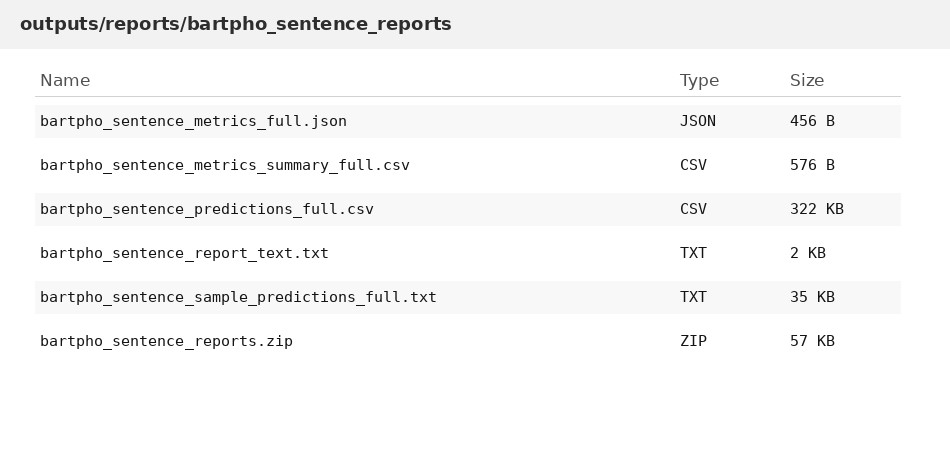
\includegraphics[width=0.78\textwidth]{figures/nlp/vsl_report_files.jpg}
\caption{Các file báo cáo được sinh sau khi đánh giá mô hình}
\label{fig:vsl-report-files}
\end{figure}

\subsubsection{Luồng xử lý chính}

Trong lớp \texttt{SentenceBuilder}, đầu vào trước hết được chuẩn hóa bằng cách loại bỏ
khoảng trắng thừa. Sau đó hệ thống xử lý theo thứ tự ưu tiên:
\begin{enumerate}
    \item nếu chuỗi đầu vào rỗng, trả về chuỗi rỗng;
    \item nếu chuỗi đầu vào khớp đúng một rule trong \texttt{sentence\_rules.json}, trả về
    câu rule tương ứng;
    \item nếu BARTpho đã được nạp thành công, gọi hàm \texttt{predict()} để sinh câu;
    \item nếu mô hình chưa có hoặc nạp lỗi, gọi \texttt{normalize\_raw\_text()} và
    \texttt{to\_sentence()} để rơi về chế độ dự phòng.
\end{enumerate}

Thứ tự này có ý nghĩa thực tiễn rất rõ:
\begin{itemize}
    \item rule-based đảm bảo các câu giao tiếp quan trọng như xin chào, xin lỗi, yêu cầu
    hỗ trợ luôn cho kết quả ổn định;
    \item BARTpho đảm nhiệm những trường hợp chuỗi gloss dài hơn hoặc linh hoạt hơn;
    \item fallback giúp hệ thống không bị ``gãy'' khi thiếu mô hình huấn luyện.
\end{itemize}

\begin{figure}[H]
\centering
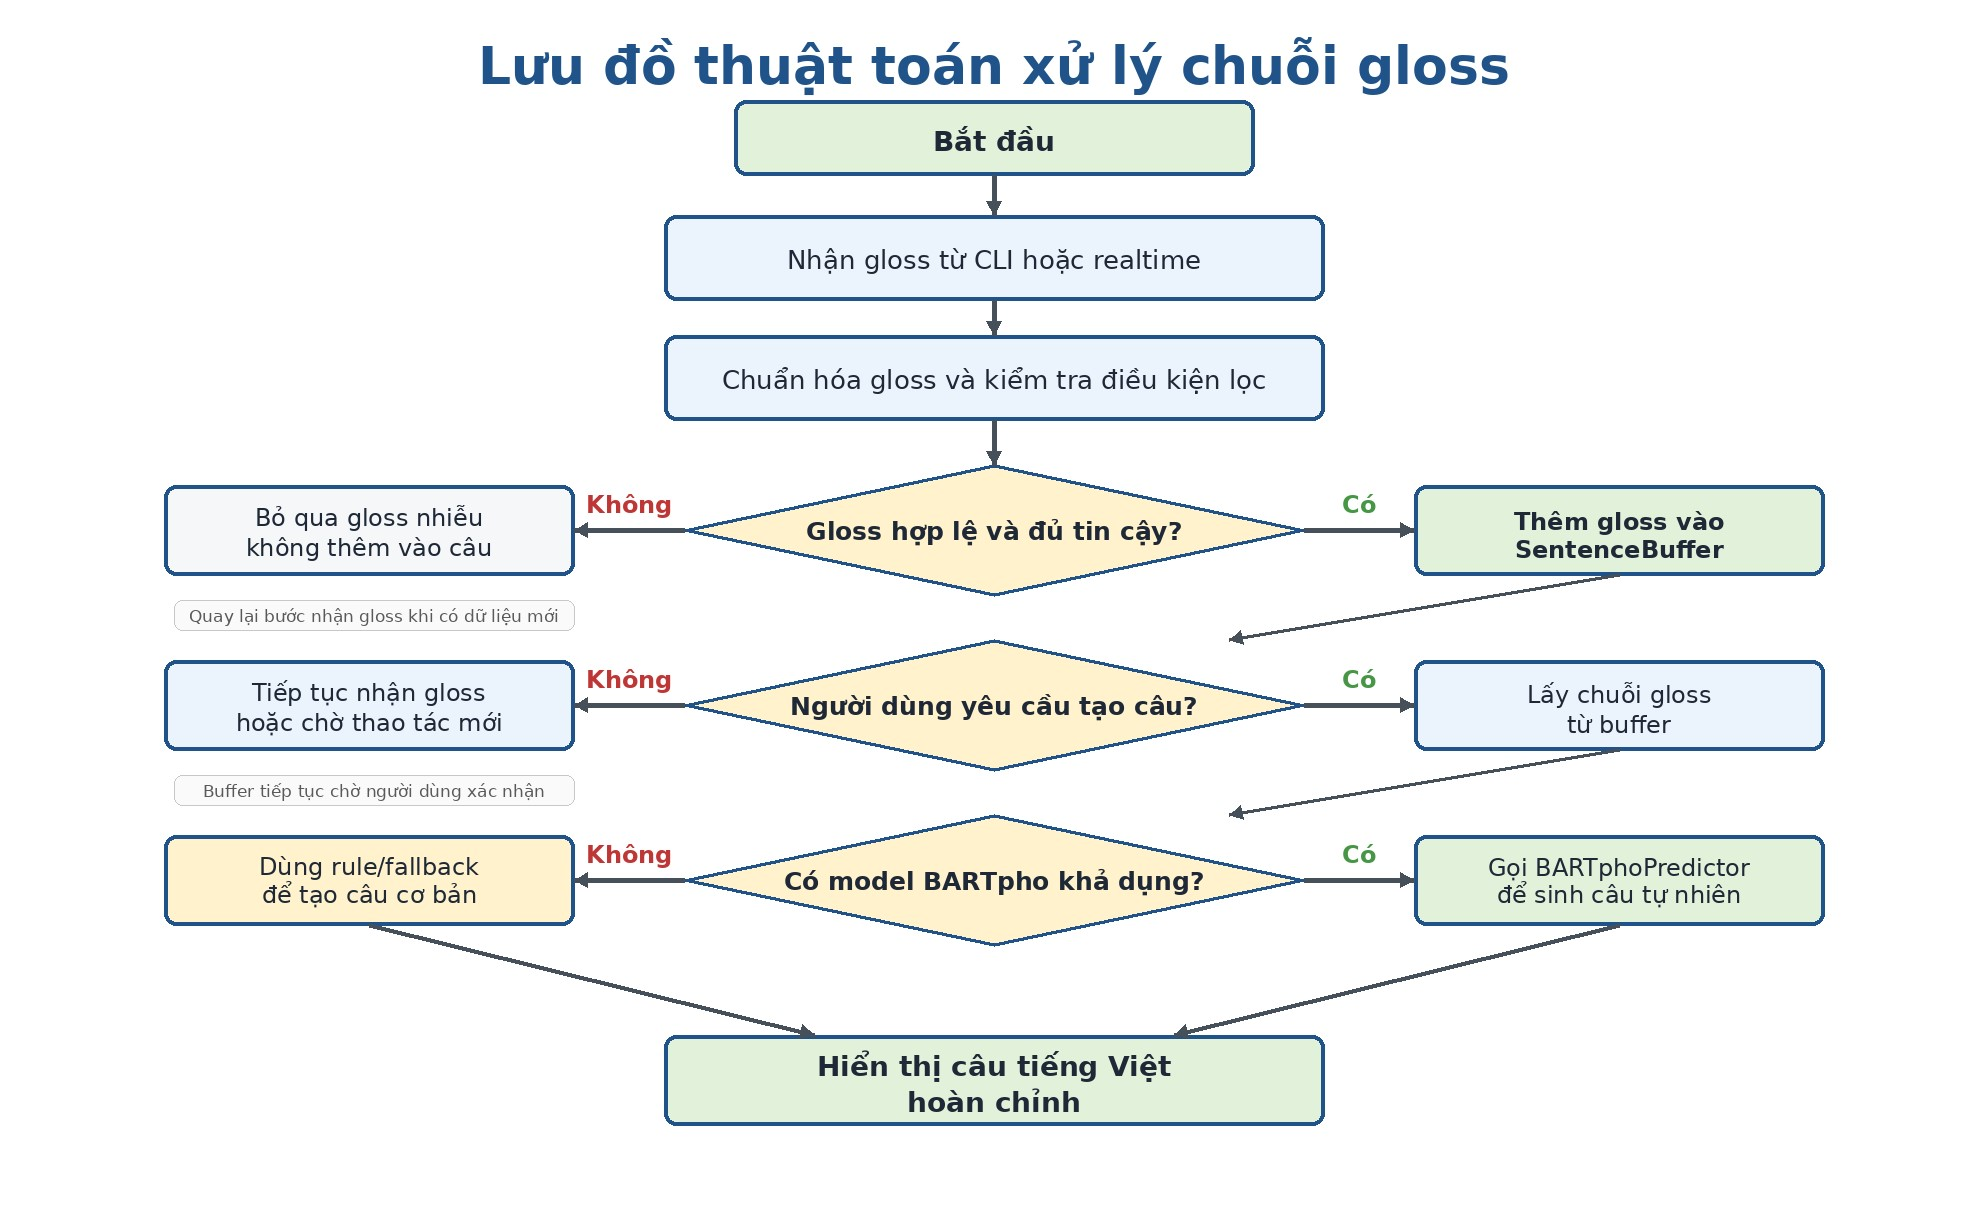
\includegraphics[width=0.94\textwidth]{figures/nlp/vsl_gloss_processing_flowchart.jpg}
\caption{Lưu đồ xử lý chuỗi gloss trong mô-đun ghép câu}
\label{fig:sentence-builder-runtime}
\end{figure}

\subsubsection{Hiện thực tầng rule-based và fallback}

Tầng rule-based được hiện thực bằng một tệp JSON đơn giản, trong đó mỗi khóa là một
chuỗi gloss chuẩn hóa, còn giá trị là câu tiếng Việt đích. Cách làm này tuy đơn giản nhưng
rất hiệu quả với các mẫu câu ngắn và các cụm ý nghĩa gần như cố định trong miền giao
tiếp hỗ trợ, ví dụ:
\begin{itemize}
    \item \texttt{xin\_chao} cho ra câu \textit{Xin chào.}
    \item \texttt{toi can giup\_do} cho ra câu \textit{Tôi cần giúp đỡ.}
    \item \texttt{toi muon uong\_nuoc} cho ra câu \textit{Tôi muốn uống nước.}
\end{itemize}

Trong trường hợp không có mô hình sinh câu, file \texttt{fallback\_corrector.py} dùng một
bảng ánh xạ token như \texttt{toi} thành \textit{tôi}, \texttt{uong\_nuoc} thành
\textit{uống nước}, \texttt{bac\_si} thành \textit{bác sĩ}. Sau khi ghép các từ lại, hệ thống tự viết hoa ký
tự đầu và thêm dấu chấm nếu cuối câu chưa có dấu kết thúc. Nhờ đó, ngay cả khi chỉ chạy
ở chế độ dự phòng, đầu ra vẫn đọc được và đủ dùng trong các demo tối thiểu.

\begin{figure}[H]
\centering
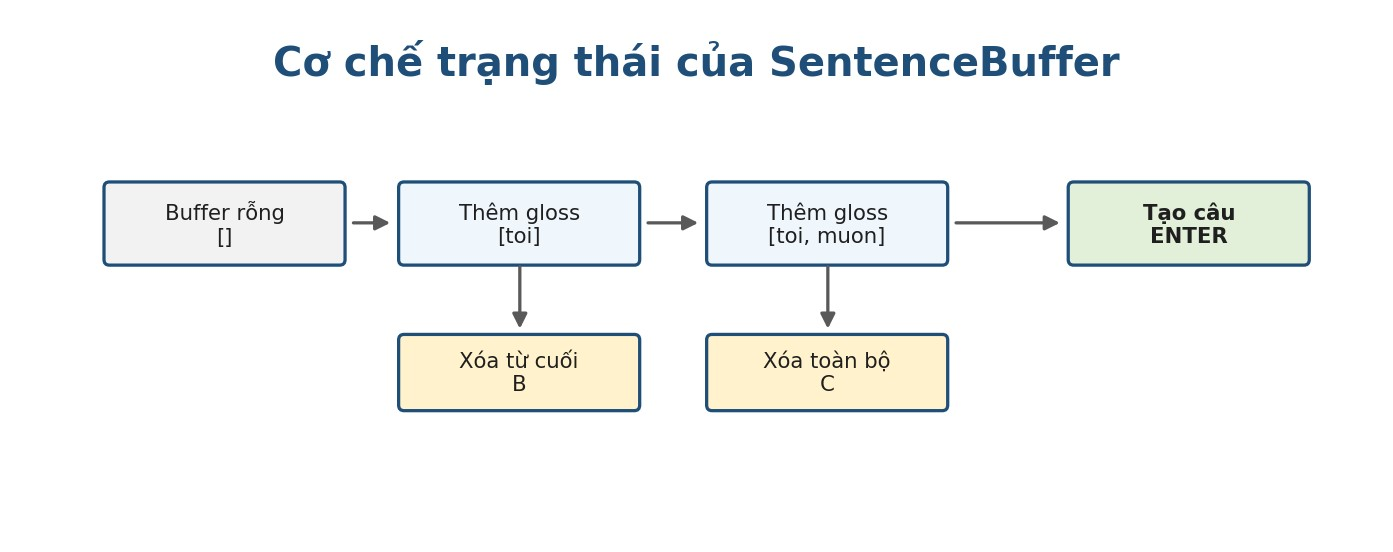
\includegraphics[width=0.82\textwidth]{figures/nlp/vsl_sentence_buffer_state_machine.jpg}
\caption{Cơ chế trạng thái của \texttt{SentenceBuffer} khi thêm, xoá và tạo câu}
\label{fig:vsl-sentence-buffer-state-machine}
\end{figure}

\subsubsection{Hiện thực suy luận bằng BARTpho}

Lớp \texttt{BartphoSentencePredictor} chịu trách nhiệm nạp mô hình từ thư mục
\texttt{models/bartpho\_sentence}. Quá trình suy luận gồm các bước:
\begin{itemize}
    \item chuẩn hóa lại chuỗi đầu vào;
    \item thêm tiền tố nhiệm vụ \texttt{chuyen\_cau\_ky\_hieu:};
    \item token hóa đầu vào với độ dài tối đa 64 token;
    \item chuyển tensor sang \texttt{cuda} nếu có GPU, ngược lại dùng CPU;
    \item sinh câu bằng \texttt{model.generate()} với \texttt{num\_beams = 4};
    \item giải mã chuỗi token sinh ra thành câu tiếng Việt hoàn chỉnh.
\end{itemize}

Điểm đáng chú ý là project giữ hoàn toàn nhất quán giữa huấn luyện và suy luận. File
\texttt{train\_bartpho.py} cũng dùng chính tiền tố \texttt{chuyen\_cau\_ky\_hieu:}, cùng
độ dài tối đa và cùng logic token hóa. Điều này giảm nguy cơ lệch phân phối dữ liệu giữa
train và inference.

\begin{figure}[H]
\centering
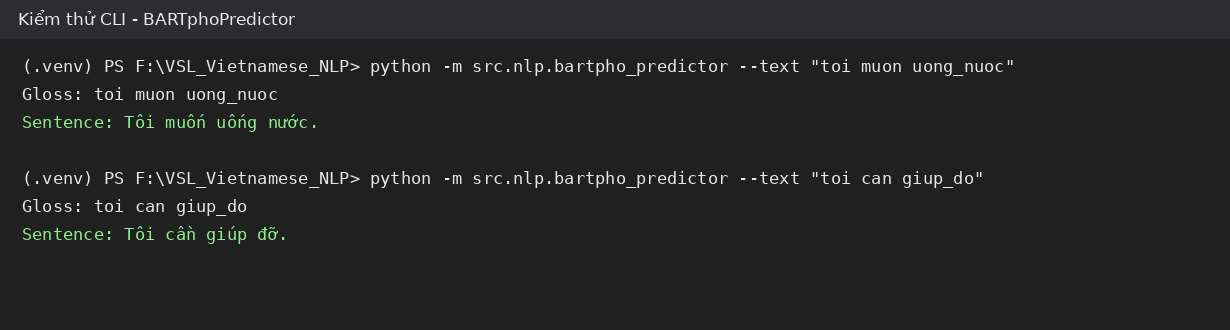
\includegraphics[width=0.78\textwidth]{figures/nlp/vsl_cli_prediction_examples.jpg}
\caption{Kiểm thử suy luận BARTpho bằng chuỗi gloss đầu vào}
\label{fig:vsl-cli-prediction-examples}
\end{figure}

\subsubsection{Khả năng tích hợp với pipeline realtime}

Mô-đun ghép câu được thiết kế để dễ tích hợp vào hệ thống thời gian thực:
\begin{itemize}
    \item giao diện đầu vào chỉ cần một chuỗi gloss đã chuẩn hóa;
    \item đầu ra là chuỗi văn bản thuần, có thể đưa tiếp sang mô-đun dịch hoặc hiển thị trực
    tiếp lên giao diện;
    \item có cơ chế suy giảm chất lượng mềm khi thiếu mô hình, thay vì dừng chương trình;
    \item logic được tách lớp rõ ràng, thuận tiện cho việc viết test riêng cho rule, model và
    fallback.
\end{itemize}

Về mặt phần mềm, đây là một quyết định quan trọng. Trong một pipeline nhiều mô-đun,
tầng NLP phải vừa đủ ``thông minh'' để cải thiện đầu ra, vừa đủ ``chắc'' để không phá vỡ
toàn bộ hệ thống khi môi trường triển khai chưa đầy đủ. Kiến trúc hiện tại đáp ứng tốt yêu
cầu đó và là nền tảng phù hợp để sau này nối trực tiếp với mô-đun nhận diện và mô-đun
dịch Việt - Lào.

